\clearpage
\subsection{Burgers 3D: provisional development panel}
\label{app:campaign:0}
\textbf{Provisional:} Audited development data with all four operator families and the same training membership. Errors use the initial-field norm and exclude time zero. Operator predictions interpolate trained time knots to the common output times. The newer operator schedules are still under evaluation. Physical refinement covers only two cases; this panel supports same-grid comparisons only.\par
\begin{table}[h]
\centering
\small
\setlength{\tabcolsep}{3pt}
\caption{33 nodes per axis; 8 development cases per method. Initial-field-normalized evolved error; same-grid reference. Each accuracy/cost pair comes from the same invocation in job 3995688. NF/NS counts nonfinite/nonstationary cases; outliers count calls above $1.5$ times the method median.}
\label{tab:campaign:0}
\resizebox{\linewidth}{!}{\input{tables/TC_development_0}}
\end{table}
\FloatBarrier
\noindent All timed arms in the main panel are included. The separately measured larger-head candidate on the same allocation is retained in the complete report, alongside representation and limited refinement diagnostics. FOM labels identify nonlinear (n) and inner linear (l) tolerances.\par
\begin{figure}[h]
\centering
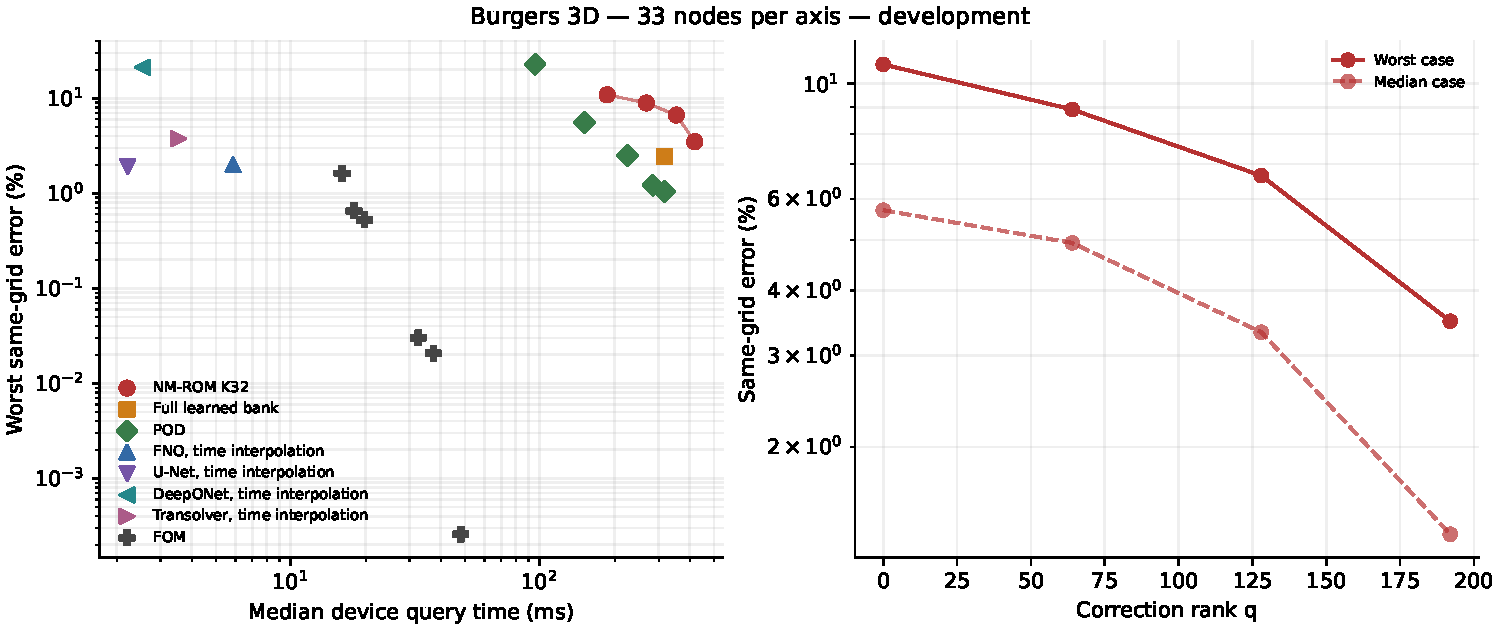
\includegraphics[width=\linewidth]{evidence/campaign-2026-09-20/burgers3d-b3d004-n33.pdf}
\caption{Provisional paired development measurements from Table~\ref{tab:campaign:0}. The right panel isolates the fixed-head correction ladder; the left retains classical controls and operator variants. Zero-error direct solves are identified separately rather than clipped onto the logarithmic error axis.}
\label{fig:campaign:0}
\end{figure}
\clearpage
\subsection{Heat 3D: provisional development panel}
\label{app:campaign:1}
\textbf{Provisional:} Audited development data with all four operator families. Errors use the current reference-field norm and exclude time zero. All recorded fits and evolved solves are stationary. The larger head improves the high-correction endpoint but retains a generalization gap; improved initialization and longer operator schedules are under evaluation. Failed direct transfer variants are retained; native-grid interpolation is charged separately. Finer-grid POD is rebuilt offline from the same training members; it is a mesh-adapted classical control, not frozen-weight transfer.\par
\begin{table}[h]
\centering
\small
\setlength{\tabcolsep}{3pt}
\caption{64 intervals per axis; 16 development cases per method. Current-reference-normalized evolved error; same-grid reference. Each accuracy/cost pair comes from the same invocation in job 3995709. NF/NS counts nonfinite/nonstationary cases; outliers count calls above $1.5$ times the method median.}
\label{tab:campaign:1}
\resizebox{\linewidth}{!}{\input{tables/TC_development_1}}
\end{table}
\FloatBarrier
\noindent The complete audited report retains smaller-head ladders, intermediate POD ranks and time-step diagnostics. Failed sampled-quadrature certificates remain in the earlier attempt and are not promoted.\par
\begin{figure}[h]
\centering
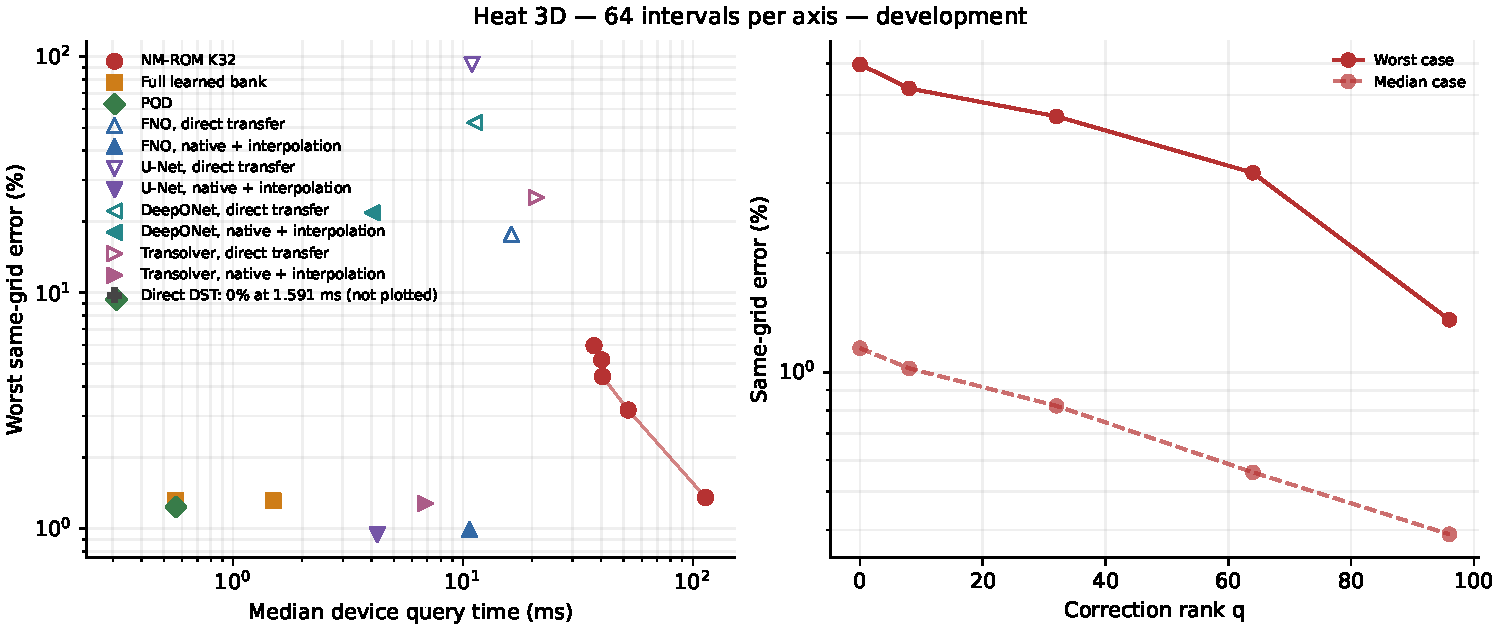
\includegraphics[width=\linewidth]{evidence/campaign-2026-09-20/heat3d-extra03-n64.pdf}
\caption{Provisional paired development measurements from Table~\ref{tab:campaign:1}. The right panel isolates the fixed-head correction ladder; the left retains classical controls and operator variants. Zero-error direct solves are identified separately rather than clipped onto the logarithmic error axis.}
\label{fig:campaign:1}
\end{figure}
\clearpage
\subsection{Poisson 3D: provisional development panel}
\label{app:campaign:2}
\textbf{Provisional:} Audited development data with all four operator families. Static weights are placed on the GPU during setup. New operator curves are still improving and longer common schedules are under evaluation. Direct transfer variants and quadrature certificates fail; preserved-domain FNO padding is a pending control. Every measured pair below shares one allocation. Finer-grid POD is rebuilt offline from the same training members; it is a mesh-adapted classical control, not frozen-weight transfer. The saved stopping records are internally consistent, but selected latent states were not retained for an independent weak-gradient audit.\par
\begin{table}[h]
\centering
\small
\setlength{\tabcolsep}{3pt}
\caption{64 intervals per axis; 16 development cases per method. Relative field error against the same-grid discrete solution. Each accuracy/cost pair comes from the same invocation in job 3995104. NF/NS counts nonfinite/nonstationary cases; outliers count calls above $1.5$ times the method median.}
\label{tab:campaign:2}
\resizebox{\linewidth}{!}{\input{tables/TC_development_2}}
\end{table}
\FloatBarrier
\noindent The complete audited report retains the K8 ladder, intermediate POD ranks, and failed sampled-quadrature diagnostics. They are not presented as missing experiments.\par
\begin{figure}[h]
\centering
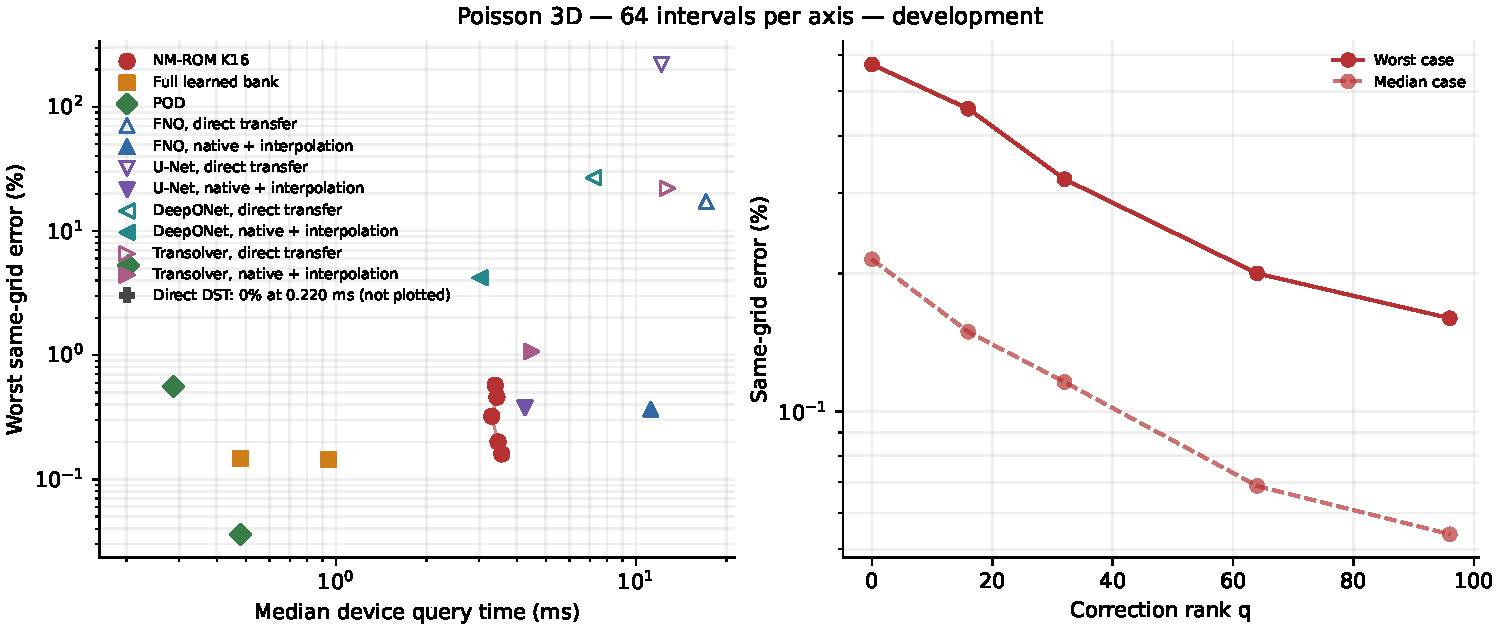
\includegraphics[width=\linewidth]{evidence/campaign-2026-09-20/poisson3d-extra03-n64.pdf}
\caption{Provisional paired development measurements from Table~\ref{tab:campaign:2}. The right panel isolates the fixed-head correction ladder; the left retains classical controls and operator variants. Zero-error direct solves are identified separately rather than clipped onto the logarithmic error axis.}
\label{fig:campaign:2}
\end{figure}
\clearpage
\subsection{Navier--Stokes 3D: provisional development panel}
\label{app:campaign:3}
\textbf{Provisional:} Independently audited new paired development measurements with all four operator families. Errors use the initial vector-field norm and exclude time zero. Learned-bank and head accuracy targets fail. Saved latent histories support sampled independent weak-gradient checks. A strict cross-run frozen-field replay gate failed and remains failed; no numerical-equivalence or implementation-speed claim is made. Augmented training and larger-bank tuning remain in progress.\par
\begin{table}[h]
\centering
\small
\setlength{\tabcolsep}{3pt}
\caption{32 periodic points per axis; 8 development cases per method. Initial-field-normalized evolved error; same-grid reference. Each accuracy/cost pair comes from the same invocation in job 3995695. NF/NS counts nonfinite/nonstationary cases; outliers count calls above $1.5$ times the method median.}
\label{tab:campaign:3}
\resizebox{\linewidth}{!}{\input{tables/TC_development_3}}
\end{table}
\FloatBarrier
\noindent All timed arms are included; the separate larger-bank snapshot-fit diagnostics remain in the complete archive. Leray projection enforces discrete incompressibility and its online cost is charged.\par
\begin{figure}[h]
\centering
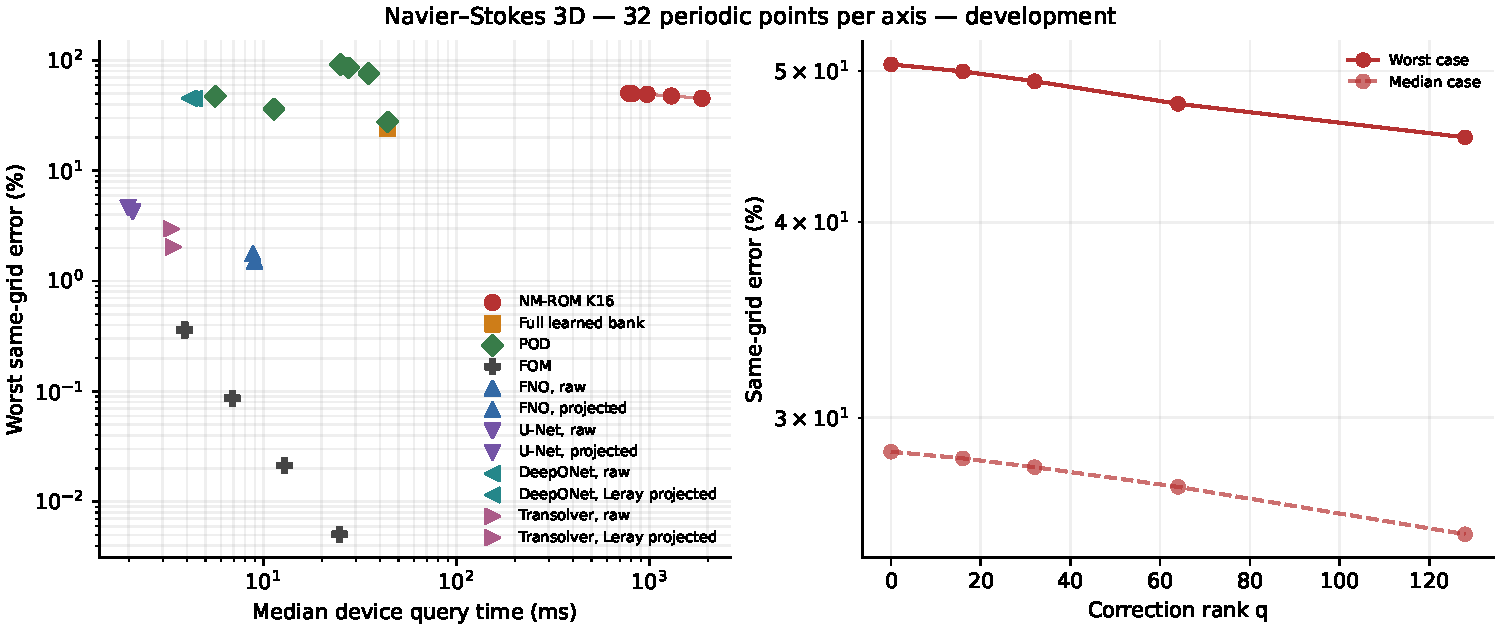
\includegraphics[width=\linewidth]{evidence/campaign-2026-09-20/ns3d-extra03-n32.pdf}
\caption{Provisional paired development measurements from Table~\ref{tab:campaign:3}. The right panel isolates the fixed-head correction ladder; the left retains classical controls and operator variants. Zero-error direct solves are identified separately rather than clipped onto the logarithmic error axis.}
\label{fig:campaign:3}
\end{figure}
